\documentclass[10pt,a4paper]{article} 
\usepackage[utf8]{inputenc}
\usepackage{amsmath} 
\usepackage{amsfonts} 
\usepackage{amssymb} 
\usepackage[all]{nowidow} 
\usepackage[style=authoryear, backend=biber, maxnames=3]{biblatex} 
\usepackage[all]{nowidow} 
\usepackage{hyperref} 
\usepackage[pdftex]{graphicx}
\usepackage[onehalfspacing]{setspace} 

\usepackage{tikz}
\usepackage{standalone}
\usepackage{eurosym}
\usepackage{ntheorem}
\theoremseparator{:}
\newtheorem{hyp}{Hypothese}
\usepackage{dcolumn}
\usepackage{graphics}
\usepackage[toc,page]{appendix}
\usepackage{booktabs,caption,fixltx2e}
\usepackage[flushleft]{threeparttable}

\usepackage[english]{babel} % for the language

\usepackage{fullpage} % this and the next one is for 1-inch margin 
\addbibresource{bib_file.bib} 
\setlength\parindent{0pt} 
\newcommand{\Title}{Religious people do not discount the future less} 
\newcommand{\Programme}{Corporate Management \& Economics}
\newcommand{\AsssignmentName}{Assignment}
\newcommand{\Name}{Samuel Pertl}
\newcommand{\MatrikelNummer}{000055998}
\newcommand{\Date}{20-12-2016}
\newcommand{\Semester}{Fall Term 2017}
\newcommand{\Supervisor}{Thor Veen}
\newcommand{\Class}{Data Science A}

\begin{document}
\pagenumbering{gobble}
\begin{centering}
\Large \textbf{Zeppelin Universität} \\
\vfill
\LARGE \textbf{\Title} \\
\vfill
\LARGE \AsssignmentName \\ %Bachelorarbeit
\Large in \\
\LARGE  \Class \\
\vfill
\begin{small}
\begin{doublespace}
	\begin{tabbing}
	Immatrikulationsnummerrrrr\=\kill
	Name:\>\Name\\
	Matriculation Nummer:\>\MatrikelNummer\\
	Semester:\>\Semester\\
	Supervisor:\>\Supervisor\\
	Date:\>\Date
	\end{tabbing}
\end{doublespace}
\end{small}



\end{centering}\vspace{1cm}
\newpage


\pagenumbering{arabic}
\tableofcontents
\listoffigures
\listoftables

\newpage

\begin{abstract}
\textcite{carter2012religious} found that religious people discount future rewards more than non-religious people. Studies by\textcite{thornton2015divine} and \textcite{benjamin2010religious} did not find such a relationship. In this study I found that religion is positively related to future discounting, indicating that religious people discount future payments more than non-religious people. However, this result is just marginally significant.
\end{abstract}
 

\section{Introduction}
As shown by \textcite{mccullough2013religion} religion is associated with several beneficial outcomes such as longer life, fewer depressive symptoms and higher school achievements. One possible beneficial real life outcome of religion could be the postponement of gratification \parencite{carter2012religious}. Delay gratification could be encouraged by religion as many religions emphasize future rewards instead of immediate gratification such as reincarnation, resurrection and immorality \parencite{carter2012religious}. Furthermore, patience has an important role in many religions \parencite{carter2012religious}. Socialization in a religious environment might therefore lead to a more patient behavior, resulting in a preference for a higher later reward instead of a instant gratification \parencite{carter2012religious}.\\
In line with the economic literature the trade-off between instant and delay gratification can be modeled through an intertemporal choice experiment. In an intertemporal choice experiment participants have to decide between an amount $x$ now and a higher amount $x+y$ later, where $y$ is positive.\\ 

% not clear what I mean by future discounting 
To my knowledge three papers have investigated the relationship between religion and future discounting so far. On the one hand, \textcite{carter2012religious} found that religious people discount future payments more than their non-religious counterparts. On the other hand, neither \textcite{thornton2015divine} nor \textcite{benjamin2010religious} observed such a relationship between religion and discounting of future rewards.\\ 

Based on the contradictory findings as well as the scarcity of the previous research more research is needed to clarify the relationship between religion and the discounting of future rewards.\\
Beside this, all three studies have major drawbacks. \textcite{carter2012religious, benjamin2010religious} use undergraduate students from the United States as their participants. According to \textcite{henrich2010weirdest} undergraduate students from "Western, Educated, Industrialized, Rich and Democratic" (WEIRD) societies - especially form the USA - are the least representative samples which substantially limits the generalization of this findings. \textcite{thornton2015divine} take this drawback into consideration and recruited their participants on the online labour market M-Turk. Even though participants from M-Turk are a more representative sample than undergraduates they are not representative enough since people who work online are - as well as undergraduates - also just a small fraction of the whole population \parencite{horton2011online}.\\

This study takes these drawbacks into consideration and uses a representative sample of the German population to investigate the relationship between future discounting and religion.\footnote{For a detailed description of the data collection see \textcite{dohmen2010risk}}
Based on the existing literature the research question for the following analysis is: 
\begin{hyp}
Religious people discount the future less than non-religious people and have therefore a stronger preference for later payments as non-religious participants
\end{hyp}

%The sample consist of a cross section of the German population. 
\section{Methods}
To measure future discounting each participant took part in an intertemporal choice experiment. For this purpose each participant received an intertemporal choice matrix with 20 rows.\footnote{Table ~\ref{tab:c} in the Appendix displays intertemporal choice matrix} For each row the participant had to decide between 100 euros "today" or a higher amount of $Y$ in 12 months \parencite{dohmen2010risk}. For all rows the early payment was 100 euros but the future payment increased by each subsequent row.\\
The first time that a participant switched from the early payment to the later payment shows to which extent the participant discounts future rewards, indicated by the internal rate of return.\footnote{A detailed description of the internal rate of return can be found by brealey2013principios} For participants who never switch from the early payment to the later one, a switching row of 21 is assumed.\\  
% why they do that 
% here I have to mention that this is not appropriat e

The response variable is the switching row, which indicates how strong a participant discounts future rewards. A higher switching row indicates that the participant discounts future payments stronger since he/she demands a higher return to give up the immediate payment for the reward in 12 months.\\
The explanatory variable is the religious affiliation of a participant. Religious affiliation is coded as a dummy variable with 1 when the participant belongs to a religious community and with 0 if this is not the case.\\
Control variables are extracted from the existing literature and are displayed in Table~\ref{tab:a}.\footnote{The exact coding of the control variables can be found in the R-script}


\begin{table}[!htbp] 
\centering 
  \caption{Control variables}\label{tab:a}
\begin{center}
\scalebox{0.7}{
\begin{tabular}{|p{5cm}|p{17cm}|}
\hline Gender & 1 = male and 0 = female \\
\hline Age  & Age in years \\
%\hline Income & Logarithm of monthly income in euros of all household members, net of taxes and benefits \\ 
%\hline Credit constraint & 1 = no credit constraint and 0 = credit constraint\\
%\hline Big Five & Openness to experience, Conscientiousness, Extraversion, Agreeableness, Neuroticism\\  
\hline
\end{tabular}}
\end{center}
\end{table}

% add the notes so 
%If monthly income was not available, income is modeled through self-reported income measured in intervals (0-750; 750-1500; 1500-2500; 2500-3500; 3500-5000: $>$5000). The interval midpoint (7500 in the case of $>$5000) function as the monthly income.\\ 

%Credit constraint is modeled through the question: "If you suddenly encounter an unforeseen situation, and had to pay an expense of 1000 euros in the next two weeks, would you be able to make the payment?". The Big Five is a psychological model that measures personality through five key dimensions: conscientiousness, extroversion, agreeableness, openness and neuroticism \parencite{dohmen2010risk}. Each personality trait is measured on a seven-point-scale with 3 question per personality trait. For each peculiarity of Big Five the scores from the three questions are added, resulting in an overall score for each Big Five. \footnote{When necessary the scores from some questions are reversed in their polarity in order to possibly achieve the maximum overall score} In order to make a statement how an individual participant's score compares with the score of the hole sample I standardize each Big Five. Therefore estimators for each personality trait have to be interpreted as a change in the switching row through an increase of the respective Big Five by one standard deviation, ceteris paribus. To control for systematic differences between male and female regarding the Big Five, each personality trait is interacted with gender \parencite{dohmen2010risk}. 


%which variables do I use and why do I use them 

In the first step the data is visualized to get an overview and observe whether the response variable switching row is normally distributed. Checking the normality provides the basis on which statistical tests can be applied. 
In a second step a Welch two-sample t-test is applied to compare the means of switching row between religious and non-religious people as the variances of these two groups are not equal. A Welch two-sample t-test is appropriate as switching row is approximately normally distributed. \footnote{For a detailed description why switching row is normal distributed see the Result Section} Although a Welch t-test is sufficient a nonparametric test (Wilcoxon-Mann-Whitney test) is conducted to verify the previous results.
In a third step a linear regression model is fitted to the data. This allows to control for variables that may have an influence on intertemporal decision making and detect whether religion still has an influence on the switching row after controlling for these variables. Forth, an analysis of variance (ANOVA) is performed to compare two regression models and decide whether the  model with more variables fits the data better than the model with less variables. Finally, I carry out a regression diagnostic and check whether the assumptions normality of residuals and  homoscedasticity are met within the linear regression.\\  

Results are interpreted in light of the conventional 5 \% significance level. For the interpretation of the linear regression the ceteris paribus clause pertains and is not mentioned again.

\section{Results}


53.8 \% of the participants are female and 46.2 \% are male with a mean of age of 46 (range: 14 - 90). Participants belong to a wide range of religious communities (Protestant: 34.8\%, Catholic: 31.4 \%, member of a different Christian denomination or religious community: 2.6\%, Islamic: 2.2\%, another religious community: 0.2\%, no religious community: 28.8\%).\\
 
Visualizing the data with a histogram (Figure~\ref{fig:a}) shows that switching row is not normally distributed since the data is highly left skewed. A Q-Q Plot as well as a Shapiro-Wilk test support this result of a non-Normal distribution of switching row (p-value $< 0.001$).\footnote{Q-Q Plot can be found in the Appendix}\\

\begin{figure}[!htbp] 
\begin{center}
\caption{Histogramm of switching row with a normal distribution}\label{fig:a}
\scalebox{0.5}{
% Created by tikzDevice version 0.10.1 on 2016-12-17 11:18:50
% !TEX encoding = UTF-8 Unicode
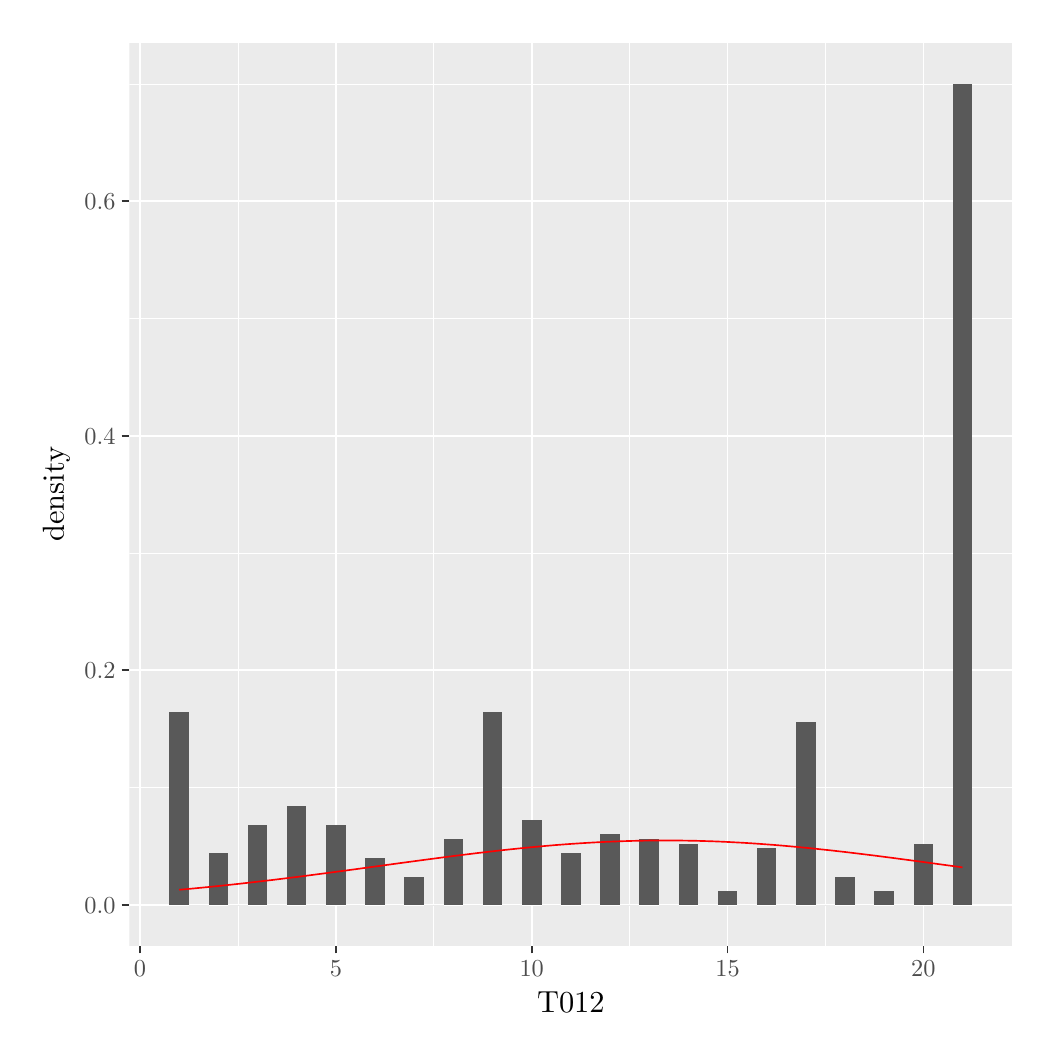
\begin{tikzpicture}[x=1pt,y=1pt]
\definecolor{fillColor}{RGB}{255,255,255}
\path[use as bounding box,fill=fillColor,fill opacity=0.00] (0,0) rectangle (361.35,361.35);
\begin{scope}
\path[clip] (  0.00,  0.00) rectangle (361.35,361.35);
\definecolor{drawColor}{RGB}{255,255,255}
\definecolor{fillColor}{RGB}{255,255,255}

\path[draw=drawColor,line width= 0.6pt,line join=round,line cap=round,fill=fillColor] (  0.00, -0.00) rectangle (361.35,361.35);
\end{scope}
\begin{scope}
\path[clip] ( 36.71, 29.59) rectangle (355.85,355.85);
\definecolor{fillColor}{gray}{0.92}

\path[fill=fillColor] ( 36.71, 29.59) rectangle (355.85,355.85);
\definecolor{drawColor}{RGB}{255,255,255}

\path[draw=drawColor,line width= 0.3pt,line join=round] ( 36.71, 86.79) --
	(355.85, 86.79);

\path[draw=drawColor,line width= 0.3pt,line join=round] ( 36.71,171.53) --
	(355.85,171.53);

\path[draw=drawColor,line width= 0.3pt,line join=round] ( 36.71,256.28) --
	(355.85,256.28);

\path[draw=drawColor,line width= 0.3pt,line join=round] ( 36.71,341.02) --
	(355.85,341.02);

\path[draw=drawColor,line width= 0.3pt,line join=round] ( 75.98, 29.59) --
	( 75.98,355.85);

\path[draw=drawColor,line width= 0.3pt,line join=round] (146.75, 29.59) --
	(146.75,355.85);

\path[draw=drawColor,line width= 0.3pt,line join=round] (217.51, 29.59) --
	(217.51,355.85);

\path[draw=drawColor,line width= 0.3pt,line join=round] (288.27, 29.59) --
	(288.27,355.85);

\path[draw=drawColor,line width= 0.6pt,line join=round] ( 36.71, 44.42) --
	(355.85, 44.42);

\path[draw=drawColor,line width= 0.6pt,line join=round] ( 36.71,129.16) --
	(355.85,129.16);

\path[draw=drawColor,line width= 0.6pt,line join=round] ( 36.71,213.90) --
	(355.85,213.90);

\path[draw=drawColor,line width= 0.6pt,line join=round] ( 36.71,298.65) --
	(355.85,298.65);

\path[draw=drawColor,line width= 0.6pt,line join=round] ( 40.60, 29.59) --
	( 40.60,355.85);

\path[draw=drawColor,line width= 0.6pt,line join=round] (111.37, 29.59) --
	(111.37,355.85);

\path[draw=drawColor,line width= 0.6pt,line join=round] (182.13, 29.59) --
	(182.13,355.85);

\path[draw=drawColor,line width= 0.6pt,line join=round] (252.89, 29.59) --
	(252.89,355.85);

\path[draw=drawColor,line width= 0.6pt,line join=round] (323.65, 29.59) --
	(323.65,355.85);
\definecolor{fillColor}{gray}{0.35}

\path[fill=fillColor] ( 51.22, 44.42) rectangle ( 58.29,113.91);

\path[fill=fillColor] ( 58.29, 44.42) rectangle ( 65.37, 44.42);

\path[fill=fillColor] ( 65.37, 44.42) rectangle ( 72.45, 63.06);

\path[fill=fillColor] ( 72.45, 44.42) rectangle ( 79.52, 44.42);

\path[fill=fillColor] ( 79.52, 44.42) rectangle ( 86.60, 73.23);

\path[fill=fillColor] ( 86.60, 44.42) rectangle ( 93.68, 44.42);

\path[fill=fillColor] ( 93.68, 44.42) rectangle (100.75, 80.01);

\path[fill=fillColor] (100.75, 44.42) rectangle (107.83, 44.42);

\path[fill=fillColor] (107.83, 44.42) rectangle (114.90, 73.23);

\path[fill=fillColor] (114.90, 44.42) rectangle (121.98, 44.42);

\path[fill=fillColor] (121.98, 44.42) rectangle (129.06, 61.37);

\path[fill=fillColor] (129.06, 44.42) rectangle (136.13, 44.42);

\path[fill=fillColor] (136.13, 44.42) rectangle (143.21, 54.59);

\path[fill=fillColor] (143.21, 44.42) rectangle (150.29, 44.42);

\path[fill=fillColor] (150.29, 44.42) rectangle (157.36, 68.15);

\path[fill=fillColor] (157.36, 44.42) rectangle (164.44, 44.42);

\path[fill=fillColor] (164.44, 44.42) rectangle (171.51,113.91);

\path[fill=fillColor] (171.51, 44.42) rectangle (178.59, 44.42);

\path[fill=fillColor] (178.59, 44.42) rectangle (185.67, 74.92);

\path[fill=fillColor] (185.67, 44.42) rectangle (192.74, 44.42);

\path[fill=fillColor] (192.74, 44.42) rectangle (199.82, 63.06);

\path[fill=fillColor] (199.82, 44.42) rectangle (206.90, 44.42);

\path[fill=fillColor] (206.90, 44.42) rectangle (213.97, 69.84);

\path[fill=fillColor] (213.97, 44.42) rectangle (221.05, 44.42);

\path[fill=fillColor] (221.05, 44.42) rectangle (228.12, 68.15);

\path[fill=fillColor] (228.12, 44.42) rectangle (235.20, 44.42);

\path[fill=fillColor] (235.20, 44.42) rectangle (242.28, 66.45);

\path[fill=fillColor] (242.28, 44.42) rectangle (249.35, 44.42);

\path[fill=fillColor] (249.35, 44.42) rectangle (256.43, 49.50);

\path[fill=fillColor] (256.43, 44.42) rectangle (263.51, 44.42);

\path[fill=fillColor] (263.51, 44.42) rectangle (270.58, 64.76);

\path[fill=fillColor] (270.58, 44.42) rectangle (277.66, 44.42);

\path[fill=fillColor] (277.66, 44.42) rectangle (284.73,110.52);

\path[fill=fillColor] (284.73, 44.42) rectangle (291.81, 44.42);

\path[fill=fillColor] (291.81, 44.42) rectangle (298.89, 54.59);

\path[fill=fillColor] (298.89, 44.42) rectangle (305.96, 44.42);

\path[fill=fillColor] (305.96, 44.42) rectangle (313.04, 49.50);

\path[fill=fillColor] (313.04, 44.42) rectangle (320.12, 44.42);

\path[fill=fillColor] (320.12, 44.42) rectangle (327.19, 66.45);

\path[fill=fillColor] (327.19, 44.42) rectangle (334.27, 44.42);

\path[fill=fillColor] (334.27, 44.42) rectangle (341.34,341.02);
\definecolor{drawColor}{RGB}{255,0,0}

\path[draw=drawColor,line width= 0.6pt,line join=round] ( 54.76, 49.83) --
	( 57.59, 50.08) --
	( 60.42, 50.35) --
	( 63.25, 50.62) --
	( 66.08, 50.90) --
	( 68.91, 51.19) --
	( 71.74, 51.49) --
	( 74.57, 51.79) --
	( 77.40, 52.10) --
	( 80.23, 52.42) --
	( 83.06, 52.75) --
	( 85.89, 53.08) --
	( 88.72, 53.41) --
	( 91.55, 53.76) --
	( 94.38, 54.11) --
	( 97.21, 54.46) --
	(100.04, 54.82) --
	(102.87, 55.19) --
	(105.71, 55.56) --
	(108.54, 55.93) --
	(111.37, 56.31) --
	(114.20, 56.69) --
	(117.03, 57.07) --
	(119.86, 57.45) --
	(122.69, 57.84) --
	(125.52, 58.23) --
	(128.35, 58.61) --
	(131.18, 59.00) --
	(134.01, 59.39) --
	(136.84, 59.77) --
	(139.67, 60.15) --
	(142.50, 60.53) --
	(145.33, 60.91) --
	(148.16, 61.28) --
	(150.99, 61.65) --
	(153.82, 62.02) --
	(156.65, 62.37) --
	(159.48, 62.72) --
	(162.31, 63.07) --
	(165.15, 63.40) --
	(167.98, 63.73) --
	(170.81, 64.05) --
	(173.64, 64.36) --
	(176.47, 64.65) --
	(179.30, 64.94) --
	(182.13, 65.22) --
	(184.96, 65.48) --
	(187.79, 65.73) --
	(190.62, 65.97) --
	(193.45, 66.19) --
	(196.28, 66.40) --
	(199.11, 66.59) --
	(201.94, 66.77) --
	(204.77, 66.93) --
	(207.60, 67.08) --
	(210.43, 67.21) --
	(213.26, 67.32) --
	(216.09, 67.42) --
	(218.92, 67.50) --
	(221.76, 67.56) --
	(224.59, 67.61) --
	(227.42, 67.64) --
	(230.25, 67.65) --
	(233.08, 67.64) --
	(235.91, 67.62) --
	(238.74, 67.57) --
	(241.57, 67.52) --
	(244.40, 67.44) --
	(247.23, 67.35) --
	(250.06, 67.24) --
	(252.89, 67.11) --
	(255.72, 66.96) --
	(258.55, 66.81) --
	(261.38, 66.63) --
	(264.21, 66.44) --
	(267.04, 66.23) --
	(269.87, 66.02) --
	(272.70, 65.78) --
	(275.53, 65.53) --
	(278.37, 65.27) --
	(281.20, 65.00) --
	(284.03, 64.72) --
	(286.86, 64.42) --
	(289.69, 64.12) --
	(292.52, 63.80) --
	(295.35, 63.48) --
	(298.18, 63.14) --
	(301.01, 62.80) --
	(303.84, 62.45) --
	(306.67, 62.10) --
	(309.50, 61.73) --
	(312.33, 61.37) --
	(315.16, 60.99) --
	(317.99, 60.62) --
	(320.82, 60.24) --
	(323.65, 59.86) --
	(326.48, 59.47) --
	(329.31, 59.08) --
	(332.14, 58.70) --
	(334.98, 58.31) --
	(337.81, 57.92);
\end{scope}
\begin{scope}
\path[clip] (  0.00,  0.00) rectangle (361.35,361.35);
\definecolor{drawColor}{gray}{0.30}

\node[text=drawColor,anchor=base east,inner sep=0pt, outer sep=0pt, scale=  0.88] at ( 31.76, 41.39) {0.0};

\node[text=drawColor,anchor=base east,inner sep=0pt, outer sep=0pt, scale=  0.88] at ( 31.76,126.13) {0.2};

\node[text=drawColor,anchor=base east,inner sep=0pt, outer sep=0pt, scale=  0.88] at ( 31.76,210.87) {0.4};

\node[text=drawColor,anchor=base east,inner sep=0pt, outer sep=0pt, scale=  0.88] at ( 31.76,295.62) {0.6};
\end{scope}
\begin{scope}
\path[clip] (  0.00,  0.00) rectangle (361.35,361.35);
\definecolor{drawColor}{gray}{0.20}

\path[draw=drawColor,line width= 0.6pt,line join=round] ( 33.96, 44.42) --
	( 36.71, 44.42);

\path[draw=drawColor,line width= 0.6pt,line join=round] ( 33.96,129.16) --
	( 36.71,129.16);

\path[draw=drawColor,line width= 0.6pt,line join=round] ( 33.96,213.90) --
	( 36.71,213.90);

\path[draw=drawColor,line width= 0.6pt,line join=round] ( 33.96,298.65) --
	( 36.71,298.65);
\end{scope}
\begin{scope}
\path[clip] (  0.00,  0.00) rectangle (361.35,361.35);
\definecolor{drawColor}{gray}{0.20}

\path[draw=drawColor,line width= 0.6pt,line join=round] ( 40.60, 26.84) --
	( 40.60, 29.59);

\path[draw=drawColor,line width= 0.6pt,line join=round] (111.37, 26.84) --
	(111.37, 29.59);

\path[draw=drawColor,line width= 0.6pt,line join=round] (182.13, 26.84) --
	(182.13, 29.59);

\path[draw=drawColor,line width= 0.6pt,line join=round] (252.89, 26.84) --
	(252.89, 29.59);

\path[draw=drawColor,line width= 0.6pt,line join=round] (323.65, 26.84) --
	(323.65, 29.59);
\end{scope}
\begin{scope}
\path[clip] (  0.00,  0.00) rectangle (361.35,361.35);
\definecolor{drawColor}{gray}{0.30}

\node[text=drawColor,anchor=base,inner sep=0pt, outer sep=0pt, scale=  0.88] at ( 40.60, 18.58) {0};

\node[text=drawColor,anchor=base,inner sep=0pt, outer sep=0pt, scale=  0.88] at (111.37, 18.58) {5};

\node[text=drawColor,anchor=base,inner sep=0pt, outer sep=0pt, scale=  0.88] at (182.13, 18.58) {10};

\node[text=drawColor,anchor=base,inner sep=0pt, outer sep=0pt, scale=  0.88] at (252.89, 18.58) {15};

\node[text=drawColor,anchor=base,inner sep=0pt, outer sep=0pt, scale=  0.88] at (323.65, 18.58) {20};
\end{scope}
\begin{scope}
\path[clip] (  0.00,  0.00) rectangle (361.35,361.35);
\definecolor{drawColor}{RGB}{0,0,0}

\node[text=drawColor,anchor=base,inner sep=0pt, outer sep=0pt, scale=  1.10] at (196.28,  5.50) {T012};
\end{scope}
\begin{scope}
\path[clip] (  0.00,  0.00) rectangle (361.35,361.35);
\definecolor{drawColor}{RGB}{0,0,0}

\node[text=drawColor,rotate= 90.00,anchor=base,inner sep=0pt, outer sep=0pt, scale=  1.10] at ( 13.08,192.72) {density};
\end{scope}
\end{tikzpicture}
}
\end{center}
\end{figure}
eine
Applying various transformation to the the variable does not result in a normal distribution of switching row and are therefore not utilized.\footnote{Logarithm, Arcsine, Square-root, Square, Reciprocal, Antilog transformations are applied and can be found in the R-script} 

According the the Central Limit Theorem (CLT), samples with a sufficient large size are approximately normal distributed and therefore parametric tests are suitable. Moreover, normality is not a requirement to fit a linear regression since just the coefficients estimates $\hat{\beta}$ have to be normal to compute confidence intervals and perform tests \parencite{lumley2002importance}. As $\hat{\beta}$ is a weighted sum of the response variable, “the CLT guarantees that it will be normally distributed if the sample size is large enough, and so tests and confidence intervals can be based on the associated t-statistic" \parencite{lumley2002importance}. However, it is questionable if the CLT applies and which sample size would be “large enough" as my sample is extremely non-Normal with a highly left skewness. \textcite{lumley2002importance} show for extremely non-Normal public health data that a sample is sufficiently large when the sample size is around 500. As my data set has a sample size of 500 observations and I see no reason why there should be a substantial difference between highly non-Normal data from the health care sector and my data parametric tests as well as a linear regression are appropriate.\\

%validity of t-test and linear regression  in sufficiently large samples depends only on assumptions about the variance of the response 

% http://stats.stackexchange.com/questions/100214/assumptions-of-linear-models-and-what-to-do-if-the-residuals-are-not-normally-di
% http://stats.stackexchange.com/questions/29731/regression-when-the-ols-residuals-are-not-normally-distributed
% http://stats.stackexchange.com/questions/29636/robust-regression-setting-the-limit-between-errors-and-influential-observations

The mean switching row for religious participants is 13.81 (sd = 7.1) and for non-religious people 12.45 (sd = 7.63). Comparing the two means with a Welch t-test shows that the two means are not significantly different and that religious people do not have a higher switching row than their non-religious counterparts (p-value: $0.066$). This is supported by a 95\% confidence interval which does include a mean difference of zero. Also a Wilcoxon-Mann-Whitney test indicates that the switching rows of religious participants are likely not shifted left or right with respect to switching row of the non-religious participants (p-value: $0.081$).\\ 

\subsection{Linear regression}
The results of the linear regression are shown in Table ~\ref{tab:b}. The intercept of first the regression model indicates the expected switching row for the non-religious participants is 12.45 (p-value $<$ 0.0001). The estimator for the dummy variable religion shows that that the expected switching row for religious participants is 1.36 higher than the switching row of non-religious participants. However, this result is not statistically significant but very close to the 5\% mark (p-value: 0.058). The F-test displays that the model statistically does not fit the data since the estimator religion is not different from zero (p-value: 0.058). The adjusted $R^2$ implies that the model explains 0.05\% of the variance of switching row but this is not statistically significant.\\

% also does not explain a lot exconomically 

The second model controls for age and gender. The intercept of 12.44 is the expected switching row for non-religious females (p-value $<$ 0.001). The estimator religion shows that the expected switching row for religious participants is 1.386 higher than the expected switching row for non-religious participants. Again, this is not statistically significant (p-value: 0.054). The estimator age implies that if we increase age by one year the expected switching row increases by 0.006. Though, this is not significant (p-value: 0.732). The F-test indicates that the model does not fit the data since all the coefficients are not different from zero (p-value: 0.197).\\

Comparing the two models with an ANOVA also shows that we should not keep the additional variables in the model as the reduction in the sum of squared residuals of 46.066 is not statistical significant and the two models are therefore not significantly different (p-value: 0.645).\\

%The estimator $log(income)$ indicates that if we increase income by 10 percent the switching row decreases by 0.223 (p-value: 0.000172).

%Participants that have a secondary-school degree have an expected switching row that is 1.92 higher than the switching row for participants who do not have a secondary-school degree (p-value: 0.044). Participants that have a no school leaving degree have an expected switching row that is 8.63 higher than the switching row for participants who have a school degree (p-value: 0.0973).

% interaction term still do not know how to interpret an interaction effect when 

 

%The adjusted $R^2$ shows that 4.958\% of the variance in switching row is explained by the model but the remaining 95.042 \% are still unexplained.


\begin{table}[!htbp] 
\centering 
\caption{Regression Results}\label{tab:b}
\scalebox{0.6}{
\label{}
\begin{tabular}{@{\extracolsep{5pt}}lD{.}{.}{-3} D{.}{.}{-3} } 
\\[-1.8ex]\hline 
\hline \\[-1.8ex] 
 & \multicolumn{2}{c}{\textit{Dependent variable:}} \\ 
\cline{2-3} 
\\[-1.8ex] & \multicolumn{2}{c}{Switching row} \\ 
\\[-1.8ex] & \multicolumn{1}{c}{(1)} & \multicolumn{1}{c}{(2)}\\ 
\hline \\[-1.8ex] 
 Religio & 1.363^{*}$ $(0.717) & 1.386^{*}$ $(0.717) \\ 
  Male &  & -0.562$ $(0.651) \\ 
  Age &  & 0.006$ $(0.018) \\ 
  Constant & 12.451^{***}$ $(0.605) & 12.436^{***}$ $(1.069) \\ 
 \hline \\[-1.8ex] 
Observations & \multicolumn{1}{c}{500} & \multicolumn{1}{c}{499} \\ 
R$^{2}$ & \multicolumn{1}{c}{0.007} & \multicolumn{1}{c}{0.009} \\ 
Adjusted R$^{2}$ & \multicolumn{1}{c}{0.005} & \multicolumn{1}{c}{0.003} \\ 
Residual Std. Error & \multicolumn{1}{c}{7.257 (df = 498)} & \multicolumn{1}{c}{7.250 (df = 495)} \\ 
F Statistic & \multicolumn{1}{c}{3.618$^{*}$ (df = 1; 498)} & \multicolumn{1}{c}{1.564 (df = 3; 495)} \\ 
\hline 
\hline \\[-1.8ex] 
\textit{Note:}  & \multicolumn{2}{r}{$^{*}$p$<$0.1; $^{**}$p$<$0.05; $^{***}$p$<$0.01} \\
\hline Standard errors are reported in the brackets  \\
\end{tabular}}
\end{table}



% label the graph 

As the two models are not statistically different I use the first regression model to analyze the assumptions of the linear regression. The regression residuals are not normally distributed since they substantially deviate form the straight line which represents a normal distribution.\footnote{Diagnostic plots (Figure ~\ref{fig:b} and Figure ~\ref{fig:c}) can be found in the Appendix} Also a histogram shows that the residuals are not normally distributed as the they do not follow the curve of the normal distribution. Non-normality of the residuals is further supported by a Shapiro-Wilk test (p-value $<$ 0.001).\\

% this should not be a problem as 

%A first step to investigate whether the variance is constant (homoscedasicity) is to plot the residuals. Plot shows that the residuals might be constant. 
% should I use the first plot or the third plot 
% do not know how to do that 
To investigate whether the variance is constant (homoscedasticity) a Breusch-Pagan test is conducted.\footnote{For a detailed description of the Breusch-Pagan test see \textcite{wooldridge2015introductory}} The Breusch-Pagan test shows that we fail to reject the null hypothesis that the variance is constant (p-value: 0.069). The p-value is very close to 5\% therefore a more detailed analysis of the variance of regression residuals is necessary.\footnote{Another instrument to detect heteroscedasticity is the White test} Nevertheless, this is not the scope of this paper and is not further investigated.\\

\section{Discussion}
The descriptive statistics as well as the linear regression shows that the switching row for religious participants is higher than the switching row of non-religious participants. This implies that religious participants discount the future more than their non-religious counterparts. All these results are not statistically significant at the conventional 5\% significance level but are very close to the 5\% mark. Hence, results could be interpreted as marginally significant. A positive relationship between religion and future discounting is controversial to the previous literature. One possible explanation could be that I use a representative sample instead of undergraduates or online laborers. More research is needed to clarify the relationship between religion and future discounting.\\

%what are the implications??, why could religious participants have a higher switching row 
%what does the diagnostic show 

This paper is not without limitations. First, the data is extremely left skewed. Although the CLT should apply it could be that the sample size is not large enough and descriptive statistics as well as linear regression are misleading. Second, the adjusted $R^2$ is very small indicating that other variables could explain switching rows better. % is that correct?? 
Third, for 35 \% of the participants a switching row of 21 is assumed as they never switch from the immediate to the later payment. This limits the validity of my analysis because I do not know the real switching row of these participants and just assume 21 as their switching row. A proper analysis should therefore just analyze the first 20 rows.\\
Future research should conduct the experiment with a larger sample size to make sure that the CLT applies. Moreover, future experimental design should increase the amount of switching rows as well as vary the extent of the discount rates to avoid extremely skewed data. Another potential application could be to fit more complex regression models such as Tobit model (controlling for censored data), robust regression methods or non-linear models to increase the fit of the linear regression. Additionally, theoretical research is needed to explain, why religion could foster immediate gratification. Finally, future work should control for more variables such as income, credit constraints, Big Five, education or cognitive ability as these variables are associated with intertemporal decision making. 


\newpage
\printbibliography


\begin{appendices}

\begin{table}[!htbp] 
\centering 
  \caption{Pay-off matrix for intertemporal choice experiment}\label{tab:c}
\begin{center}
\scalebox{0.7}{
\begin{tabular}{p{2cm}|p{3cm}|p{2cm}|p{3cm}}
  & today & or & in 12 months\\
\hline 1 & 100.00 & & 102.50\\
\hline 2 & 100.00 & & 105.10 \\
\hline 3 & 100.00 & & 107.60 \\
\hline 4 & 100.00 & & 110.20 \\
\hline 5 & 100.00 & & 112.80 \\
\hline 6 & 100.00 & & 115.50 \\
\hline 7 & 100.00 & & 118.20 \\
\hline 8 & 100.00 & & 121.00 \\
\hline 9 & 100.00 & & 123.70 \\
\hline 10 & 100.00 & & 126.50 \\
\hline 11 & 100.00 & & 129.30 \\
\hline 12 & 100.00 & & 132.20 \\
\hline 13 & 100.00 & & 135.10 \\
\hline 14 & 100.00 & & 138.00 \\
\hline 15 & 100.00 & & 141.00 \\
\hline 16 & 100.00 & & 144.00 \\
\hline 17 & 100.00 & & 147.00 \\
\hline 18 & 100.00 & & 150.00 \\
\hline 19 & 100.00 & & 153.10 \\
\hline 20 & 100.00 & & 156.20\\
\hline
\end{tabular}}
\end{center}
\end{table}


\begin{figure}
    \centering
    \begin{minipage}{0.45\textwidth}
\caption{Histogram of regression residuals with normal distribution}\label{fig:b}
        \includegraphics[width=0.9\textwidth]{final.tex} % first figure itself
        
    \end{minipage}\hfill
    \begin{minipage}{0.45\textwidth}
\caption{Q-Q Plot of regression residuals}\label{fig:c}
        \includegraphics[width=0.9\textwidth]{final2.tex} % second figure itself
        
    \end{minipage}
\end{figure}


\end{appendices}


\end{document}
